\chapter{HERRAMIENTAS DE DESARROLLO}

\section{TICs en la Educaci\'{o}n}

Es importante entender que las TICs \footnote{TICS: Tecnolog\'{i}as de la 
Informaci\'{o}n y de Comunicaci\'{o}n \cite{severin2013enfoques}} no son s\'{o}lo herramientas, uno de ellos
se tiene cuando la persona queda excluida del acceso y uso de las TICs es como si
estubiera dejando de interactuar con el mundo exterior, incluso se habla de que 
el acceso tecnolog\'{i}a y conectividad como un derecho hacia un bien b\'{a}sico.

El primer foco de la atenci\'{o}n definido es el considerar la manera en que las TICs
favorecen el desarrollo de nuevas pr\'{a}cticas educativas, m\'{a}s pertinenetes y eficaces,
lo que incluye fortalecer el protagonismo que tienen los docentes en los cambios
educativos.\cite{severin2013enfoques}

\section{Educaci\'{o}n y virtualidad: hacia un espacio de vivencia de valores}

La relaci\'{o}n entre la educaci\'{o}n y la virtualidad es de creatividad. La 
educaci\'{o}n a trav\'{e}s de la web explica las did\'{a}ctivas de cualquier 
acci\'{o}n educativa. 

Educaci\'{o}n y virtualidad se complementan para que la educaci\'{o}n pueda 
disfrutar de las posibilidades creativas de la virtualidad con la mejora de sus
procesos y las acciones encaminadas a la ense\~{n}anza y al aprendizaje, mientras
que la virtualidad se beneficia de la metodolog\'{i}a necesaria en algunos casos,
como cuando la finalidad sobrepasa la mera informaci\'{o}n.
\cite{duart2000aprender}

\section{Web 2.0}

Sin embargo, algunas de las caracter\'{i}sticas t\'{i}picas asociadas con los sitios
Web 2.0 las siguientes:

\begin{itemize}

\item \textbf{El uso compatible con los est\'{a}ndares HTML y CSS} Esto permite a
 los sitios de trabajo a trav\'{e}s de muchas plataformas, formas y ayuda con la
 accesibilidad.
\item \textbf{El Uso de Ajax para proveer una interfaz usuario rica} Mediante la
realizaci\'{o}n operaciones triviales de fondo usando XMLHttpRequest 
\footnote{XMLHttpRequest: Define una API que proporciona un gui\'{o}n 
funcionalidad de cliente para transferir datos entre un cliente y un servidor 
\cite{xmlHttpRequest}} , p\'{a}ginas web pueden ser m\'{a}s funcional e 
intuituva.
\item \textbf{Compartiendo datos mediante Web feeds y servicios web} Los
usuarios les gusta agregar muchos feeds a recibir f\'{a}cilmente actualizaci\'{o}nes
de contenido de sus sitios favoritos con v\'{i}nculos Web.
\item \textbf{La Incorporaci\'{o}n de herramientas en redes sociales} Blogs y foros 
puede permitir a los usuarios comunicarse entre s\'{i}.
	
\end{itemize}

Aunque ninguna de estas caracter\'{i}sticas o aspectos del desarrollo son nuevos,
utilizamos la Web 2.0 t\'{e}rmino para describir la actual generaci\'{o}n de sitios
web que hacen un buen uso de HTML y CSS, mientras que tal vez mejorar su interfaz
con el Ajax y herramientas de redes sociales.\cite{zervaas2007practical}

\section{Arquitectura Cliente/Servidor}

Arquitecturas cliente-servidor son generalmente consideradas como arquitecturas
de sistemas distribuidos, pero el modelo l\'{o}gico de servicios independientes
que se ejecutan en servidores separados puede implementarse en un solo equipo.
Una vez m\'{a}s, un beneficio importante es la separaci\'{o}n e independencia.
Los servicios y servidores se pueden cambiar sin afectar otras partes del sistema.

Los clientes pueden tener que saber los nombres de los servidores disponibles y
los servicios que ellos proveen. Sin embargo, los servidores no necesitan conocer
la identidad de los clientes o c\'{o}mo muchos clientes tienen acceso a sus
servicios. Los clientes acceden a los servicios prestados por un servidor a 
trav\'{e}s de llamadas a procedimientos remotos utilizando un protocolo de 
petici\'{o}n-respuesta como el http protocolo utilizando en la WWW, Esencialmente,
un cliente realiza una solicitud a un servidor y espera que reciba una respuesta.

Figura \ref{Una arquitectura cliente-sevidor para una filmoteca} es un ejemplo de
un sistema que se basa en el modelo cliente-servidor. Esta es un sistema basado en
la web multi-usuario para proporcionar una biblioteca de cine y  fotograf\'{i}a.
En este sistema, varios servidores de gesti\'{o}n, se muestran los diferentes tipos de
medios.\cite{sommerville2011software}

\begin{figure}[!htb]
	\centering
	\fbox{
		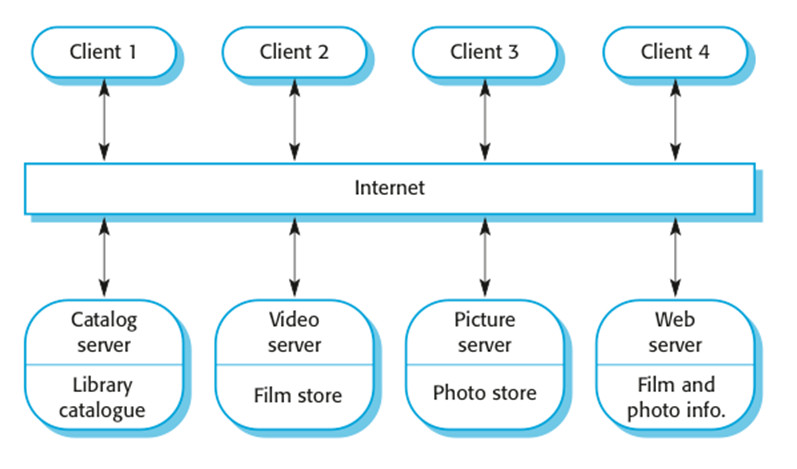
\includegraphics[scale=0.5]{architectureClientServer}
	}
	\caption{Una arquitectura cliente-sevidor para una filmoteca}
	\source{fuente: \cite{sommerville2011software}}
	\label{Una arquitectura cliente-sevidor para una filmoteca}
\end{figure}

\subsection{Patr\'{o}n Dise\~{n}o: Modelo Vista Controlador}

La idea de los patrones como una forma de presentar, compartir y reutilizar el
conocimiento sobre sistemas de software ahora se utiliza ampliamente.

Usted puede pensar en un patr\'{o}n arquitect\'{o}nico como una estilizada 
descripci\'{o}n, abstracta de buena pr\'{a}ctica, que ha sido probada en 
diferentes sistemas y entornos. Asi que, un patr\'{o}n arquitect\'{o}nico
debe describir una organizaci\'{o}n del sistema que ha sido con \'{e}xito
en los sitemas anteriores. Debe incluir informaci\'{o}n de cu\'{a}ndo es
y no es apropiado utilizar ese patr\'{o}n, y los patrones de puntos fuertes
y d\'{e}biles.

Figura \ref{Arquitectura de aplicaciones Web utilizando el patr\'{o}n MVC} muestra
una posible arquitectura de tiempo ejecuci\'{o}n cuando este patr\'{o}n se utiliza
para la gesti\'{o}n de la interacci\'{o}n en un sistema basado en la web.

En una secci\'{o}n corta de un cap\'{i}tulo general, es imposible describir todos
los patrones gen\'{e}ricos que se pueden utilizar en el desarrollo de software.
M\'{a}s bien, les presento algunos ejemlos seleccionados de los patrones que se
utilizan ampliamente y que la captura de los buenos principios de dise\~{n}o 
arquitect\'{o}nico. He incluido algunos ejemplos m\'{a}s de los patrones 
arquitect\'{o}nicos gen\'{e}ricos en las p\'{a}ginas web del libro.
\cite{sommerville2011software}

\begin{minipage}{1.0\textwidth}
	\centering
	\fbox{
		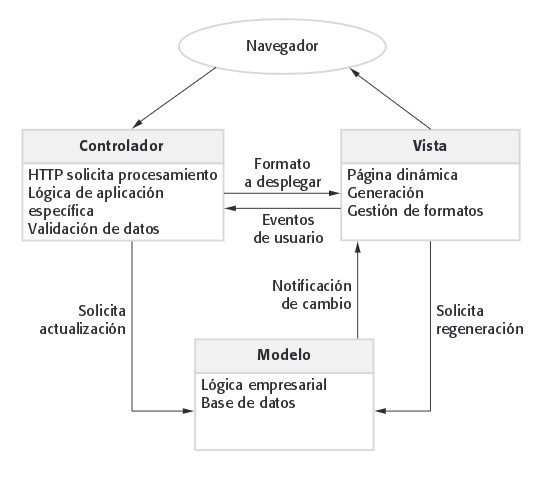
\includegraphics[scale=0.8]{mvcPattern}
	}
	\captionof{figure}{Arquitectura de aplicaciones Web utilizando el patr\'{o}n MVC}
	\source{fuente: \cite{sommerville2011software}}
	\label{Arquitectura de aplicaciones Web utilizando el patr\'{o}n MVC}
\end{minipage}

\begin{itemize}

\item \textbf{Dise\~{n}o del Proyecto}

Se toma como patr\'{o}n de Dise\~{n}o Modelo Vista Controlador como base para 
extender la funcionalidad de un Controlador denominado Manager la cual realiza
una abstracci\'{o}n de funcionalidad y reuso esta definido en la Figura 
\ref{Arquitectura Extendida MVCM}

\begin{minipage}{1.0\textwidth}
	\centering
	\fbox{
		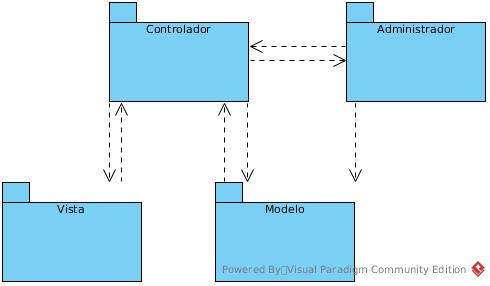
\includegraphics[scale=0.5]{mvcm}
	}
	\captionof{figure}{Arquitectura Extendida MVCM}
	\source{fuente: (Elaboraci\'{o}n Propia)}
	\label{Arquitectura Extendida MVCM}
\end{minipage}


\end{itemize}

\section{PHP}

PHP siempre ha sido un lenguaje que es especificamente \'{u}til para la 
programaci\'{o}n web. Eso sigue siendo, y con PHP5, se ha criado al d\'{i}a y
se estableci\'{o} un lenguaje que es totalmente compatible con los modernos 
m\'{e}todos orientados a objectos, pr\'{a}cticas y principios. 

Versi\'{o}n 5 de PHP \footnote{PHP: Hypertext Processor \cite{reiersol2007php}} 
es, cuanto otras cosas, un intento de hacer el uso de estos conceptos y 
metodol\'{o}gicas herramientas en PHP.\cite{reiersol2007php}

\subsection{Yii Framework}

Con Yii, los conceptos m\'{a}s importantes son Programaci\'{o}n orientada a objetos
(POO) y el patr\'{o}n Modelo-Vista-Controlador (MVC).

A diferencia de otros frameworks \footnote{framework: Es un conjunto de recursos
y herramientas para desarrolladores de software para crear y gestionar 
aplicaciones web, servicios web y sitios web. \cite{framework}} , Yii siempre ha
requerido la versi\'{o}n 5 de PHP. Esto significa, ya que PHP 5 tiene una 
estructura objeto sumamente mejorada y avanzada en comparaci\'{o}n con el 
mayores PHP 4. \cite{ullman2013yii}

\textbf{Extensiones Yii}

Se define extensiones como una abstracci\'{o}n de funcionalidad espec\'{i}fica, el
mismo puede ser utilizado en sistemas o applicaciones web: Envio de correo, 
autentificaci\'{o}n por red social, dise\~{n}o web responsivo, etc.

\begin{enumerate}

\item \textbf{Booster}

YiiBooster es una colecci\'{o}n de widgets \footnote{widgets: Es un elemento 
de una interfaz gr\'{a}fica de usuario que muestra informaci\'{o}n o 
proporciona una forma espec\'{i}fica para un usuario interactuar con el sistema
operativo o una aplicaci\'{o}n \cite{widget}} que faciliten la tarea de 
desarrollar aplicaciones Yii, as\'{i} como, dando a su aplicaci\'{o}n un poco 
de impulso. B\'{a}sicamente, Booster fuerza a los retos m\'{a}s comunes que los
desarolladores Yii enfrentan al tratar de mejorar sus aplicaciones. \cite{booster}

\item \textbf{CascadeDropDown}

Es simple de utilizar la extensi\'{o}n el plugin de JQuery JQuery-cascada para
rellenar los datos de una lista desplegable depende de un ajax/ getJSON-llamada.
 \cite{cascadedropdown}

\item \textbf{Efeed}

RSS Escritor Generador de extensi\'{o}n para crear tus feeds. Actualmente soporta
RSS 1.0, RSS 2.0 y ATOM 1.0. \cite{efeed}

\item \textbf{Hoauth}

Proveedor yii-oauth sencilla integraci\'{o}n con la red social, la autorizaci\'{o}n
lib Hybridauth \footnote{Hybridauth: Meta HybridAuth es actuar como un api 
abstracta entre la aplicaci\'{o}n y diversos apis sociales e identidades 
proveedores como Facebook, Trwiter y Google \cite{hybridauth}} en Yii. \cite{hoauth}

\item \textbf{Image}

Proporciona m\'{e}todos para la manipulaci\'{o}n din\'{a}mica de las im\'{a}genes.
Varios formatos de imagen como JPG, PNG, GIF y puede cambiar de tama\~{n}o, recortar,
rotar. \cite{image}

\item \textbf{MediaElement}

Esta extensi\'{o}n le permite agregar HTML5 reproductor de audio y v\'{i}deo 
utilizando la biblioteca MediaElementJS para su proyecto Yii. \cite{mediaelement}

\item \textbf{Yii-Image-Zoomer}

Es flexible, eficiente, m\'{a}s peque\~{n}o, tiene m\'{a}s funciones y m\'{a}s
robusta, la compatibiliadad entre navegadores. \cite{yiiImageZoomer}

\item \textbf{YiiMailer}

Extensi\'{o}n Yii para el env\'{i}o de mensajes de correo electr\'{o}nico HTML
con dise\~{n}os utilizando PHPMailer \footnote{PHPMailer: Es una de las 
bibliotecas de PHP de c\'{o}digo abierto m\'{a}s populares para enviar mensajes
de correo electr\'{o}nico \cite{phpMailer}} \cite{yiiMailer}

\end{enumerate}


\section{JavaScript} 

JavaScript es el lenguaje de programaci\'{o}n de la Web. La inmensa mayor\'{i}a
de la p\'{a}gina web moderna utiliza JavaScript y todos los modernos navegadores
web en ordenadores de sobremanera, consolas de juegos, mesas y tel\'{e}fonos 
inteligentes incluyen int\'{e}rpretes de JavaScript, haciendo JavaScript m\'{a}s
lenguaje de programaci\'{o}n  omnipresente en la historia. JavaScript es parte de
la tr\'{i}ada de tecnolog\'{i}as que todos los desarrolladores web deben aprender:
HTML para especificar el contenido de p\'{a}ginas web, CSS para especificar la 
presentaci\'{o}n de las p\'{a}ginas web y JavaScript para especificar el comportamiento
de las p\'{a}ginas web. \cite{flanagan2006javascript}

\subsection{JQuery}

JQuery es una biblioteca JavaScript de c\'{o}digo abierto que simplifica las 
interacciones entre un Documento HTML, o m\'{a}s precisamente el Documento 
Object Model (tambi\'{e}n conocido como el DOM), y JavaScript.

Espec\'{i}ficamente, JQuery simplifica documento HTML de desplazamiento y la 
manipulaci\'{o}n, manejo de eventos del navegador, animaciones DOM, interacciones
Ajax y cross-browser desarrollo JavaScript.\cite{lindley2009jquery}

\section{HTML5}

HTML fue dise\~{n}ado originalmente para, compartir est\'{a}tica documento basado
en texto en el Internet. Con el tiempo, ya que los usuarios de Internet y los 
dise\~{n}adores quer\'{i}an m\'{a}s interactividad en su documento HTML, comenzaron
a mejorar estos documentos, a\~{n}adiendo funcionalidad forma y capacidades tempranas
\textquotedblleft portal\textquotedblright tipo. Ahora, estas colecciones de 
documentos est\'{a}ticos, o de los sitios web, se aparecen m\'{a}s a las aplicaciones
web, basado en los principios del rico escritorio de aplicaciones cliente/servidor.
Estas aplicaciones web est\'{a}n siendo utilizadas en la mayor de dispositivos: 
ordenador, port\'{a}tiles, tel\'{e}fonos inteligentes, tabletas de la gama.

HTML5 hace que las aplicaciones web m\'{a}s usables, as\'{i}, ya que elimina la
necesidad para los plugins. \cite{wang2013definitive}


\section{CSS}

Los usuarios deben ser capaces de acceder a su contenido sin importar qu\'{e} 
dispositivo utilizan o qu\'{e} software est\'{a} en esos dispositivos. CSS 
permite a los desarrolladores de bien c\'{o}mo se ve el contenido, incluyendo 
m\'{e}todos para la costura o la presonalizaci\'{o}n de la presentaci\'{o}n del
contenido basado en el dispositivo. Por ejemplo, los usuarios pueden acceder a su
contenido a trav\'{e}s de un navegador en un netbook, un navegador en un t\'{e}lefono,
en su TV, con un lector de pantalla, como una presentaci\'{o}n, o incluso impreso
en formato PDF. CSS proporcina mecanismos de estafa arrastre la apariencia o 
presentaci\'{o}n de su contenido, no importa el dispositivo.\cite{weyl2012s}

\subsection{Bootstrap}

En los dias anteriores de Twitter, los ingenieros utilizan casi cualquier 
biblioteca que estaban familiarizados para satisfacer las necesidades de 
front-end. Las incoherencias entre las aplicaciones individuales hechas dif\'{i}ciles
de escalar y mantener ellos. Bootstrap comenz\'{o} como una respuesta a estos 
desaf\'{i}os y se aceler\'{o} r\'{a}pidamente durante la primera semana Hack de
Twitter. A finales de Hack semana tuvimos llegado a una versi\'{o}n estable que
los ingenieros podr\'{i}an utilizar en toda la compa\~{n}ia.\cite{spurlock2013bootstrap}

\subsection{CSS3}

Hasta el momento, el Grupo de Trabajo de CSS en el W3C ha comenzado a trabajar 
en m\'{a}s de 40 m\'{o}dulos de CSS. Agunos m\'{o}dulos, como selectores, 
espacios de nombres, Color y Medios de consultas, se considera estable y son ya
sea en Candidata a Recomendaci\'{o}n o el estado de recomendaci\'{o}n. El primer
m\'{o}dulo se convierta en una Recomendaci\'{o}n del W3C fue el CSS3 M\'{o}dulo
de color, publicado el mismo d\'{i}a que la especificaci\'{o}n CSS 2.1 se convirtio
en una recomendaci\'{o}n. El trabajo en diferentes m\'{o}dulo ha progresado a 
diferentes velocidades. Los bloqueos en un m\'{o}dulos ha progresado y se sostiene
cualquier otro m\'{o}dulo.\cite{spurlock2013bootstrap}

\section{Git}

El control de versiones es un sistema que registra cambios en un archivo o conjunto
de archivos con el tiempo para que pueda recuperar versiones especif\'{i}cas mas tarde.

Si usted es un dise\~{n}ador gr\'{a}fico o web y desea mantener todas las versiones
de una imagen o el dise\~{n}o (que usted sin duda que desee), un sistema de control
de versiones (VCS) es una cosa muy aconsejable utilizar. Te permite revertir los
archivos de nuevo a un estado anterior, revertir todo el proyecto de nuevo a un
estado anterior, comparar cambios en el tiempo, a ver qu\'{i}en dura modificado
algo que podr\'{i}a ser la causa de un problema, que se present\'{o} un problema
y cuando, y m\'{a}s.\cite{chacon2009pro}

\section{Pivotal Tracker}

Es una herramienta simple, basado en la historia de planificaci\'{o}n del proyecto
que permite a los equipos a colaborar y reaccionan instant\'{a}neamente a los 
cambios del mundo real. Se basa en m\'{e}todos de desarrollo de software \'{a}giles,
pero se puede utilizar en una variedad de tipos de proyectos. Rastreador te libera
para concentrarse en las cosas, sin empantanarse, manteniendo sus planes en 
sincron\'{i}a con la realidad. \cite{pivotalTracker}